\begin{enunciado}{\ejercicio}
  Sea $w = e^{\frac{2\pi}{3}i}$ raíz cúbica de la unidad y
  sea $(z_n)_{n \en \naturales}$ la sucesión de números
  complejos definida por:
  $$
    z_1 = 1+w  \ytext  z_{n+1} =
    \conj{1 + z_n^2},\, \paratodo n \en \naturales.
  $$

  Probar que para todo $n \en \naturales$ vale que
  $z_n =
    \llave{ll}{
      e^{\frac{2\pi}{6}i}  & \text{si $n$ impar}\\
      e^{-\frac{2\pi}{6}i}  & \text{si $n$ par}
    }$. Concluir que $z_n \en G_6$ para todo $n \en \naturales$.
\end{enunciado}

\begin{minipage}{0.75\textwidth}
  Hay que probar por inducción. Quiero probar:\par
  $p(n) :
    z_n =
    \llave{ll}{
      e^{\frac{2\pi}{6}i}  & \text{si $n$ impar}\\
      e^{-\frac{2\pi}{6}i}  & \text{si $n$ par}
    } \paratodo n \en \naturales$ \par

  \textit{Caso base: }\par

  $\llave{l}{
      p(1) : z_1 = 1 + e^{\frac{2\pi}{3}i} = 1 -\frac{1}{2} + i \frac{\sqrt{3}}{2} = \frac{1}{2} + i \frac{\sqrt{3}}{2} =  e^{\frac{\pi}{3}i} \Tilde\\
      p(2) : z_2 = \conj{ 1 + z_1^2} = \conj{ 1 + e^{\frac{2\pi}{3}i} } = 1 + e^{-\frac{2\pi}{3}i} = e^{-\frac{\pi}{3}i} \Tilde
    }$\par

  \textit{Paso inductivo: }\par

  $\llave{l}{
      p(2k) : z_{2k} = e^{-\frac{\pi}{3}i} \text{ Verdadero } \entonces p(2k+2) \  \text{¿Verdadero?}\\
      p(2k+1) : z_{2k+1} = e^{\frac{\pi}{3}i} \text{ Verdadero } \entonces p(2k+3) \  \text{¿Verdadero?}
    }$\par

  $\llave{l}{
      z_{2k+2} = \conj{ 1 + z_{2k+1}^2 }
      \Sii{HI} z_{2k+2} =
      \conj{ 1 + e^{\frac{2\pi}{3}i} } =
      \conj{ e^{\frac{\pi}{3}i} } =
      e^{-\frac{\pi}{3}i} \Tilde
      \\
      z_{2k+3} = \conj{ 1 + z_{2k+2}^2 }
      \Sii{HI} z_{2k+3} =
      \conj{ 1 + e^{-\frac{2\pi}{3}i} } =
      \conj{ e^{-\frac{\pi}{3}i} } =
      e^{\frac{\pi}{3}i} \Tilde
    }$\par

  Dado que $p(1), p(2), p(2k),p(2k+1),p(2k+2),p(2k+3)$ resultaron ser verdaderas, entonces
  por el principio de inducción se concluye que $p(n)$ también lo es $\paratodo n \en \naturales$.\par
  Dado que la sucesión $z_n$   tiene solo 2 imágenes, para cualquier $n \en \naturales$ y teniendo en cuenta
  que $e^{-i\frac{2\pi}{6}} = e^{i\frac{2\pi}{6}\cdot 5} \en G_6\ \paratodo n \en \naturales$
\end{minipage}
\begin{minipage}{0.3\textwidth}
  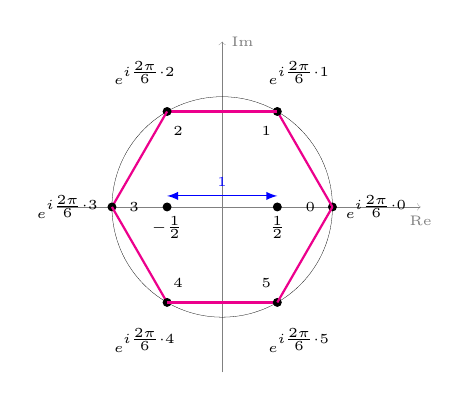
\begin{tikzpicture}[baseline=0,scale = 1.4, every node/.style={font=\tiny}]
    \draw[ultra thin,->,gray] (-1.5,0) -- (1.8,0) node[below] {Re};
    \draw[ultra thin,->,gray] (0,-1.5) -- (0,1.5) node[right] {Im};
    \draw[ultra thin] (0,0) circle (1);
    \filldraw[thin] (-.5,0) circle (1pt) node[below] {$-\frac{1}{2}$}; % Added the origin
    \filldraw[thin] (.5,0) circle (1pt) node[below] {$\frac{1}{2}$}; % Added the origin
    \draw[latex-latex, blue] (-.5,0.1) -- (0.5,0.1) node[midway, above]{ 1};
    \foreach \x in {0,...,5} {
        \filldraw (\x*360/6:1) circle (1pt) ;
        \filldraw (\x*360/6:0.8) node { $\x$};
        \filldraw (\x*360/6:1.4) node { $e^{i \frac{2\pi}{6} \cdot \x}$};
        \ifnum\x<6
          \draw[thick, magenta] (\x*360/6:1) -- ({(\x+1)*360/6}:1);
        \fi
        % \ifnum\x<3
        % 	\draw[thick, cyan] ({\x*360/3+360/3}:1) -- ({(\x+1)*360/3+360/3}:1);
        % \fi
      }
  \end{tikzpicture}
\end{minipage}
